% SPDX-FileCopyrightText: 2026 Niels Bonde Jensen
% SPDX-License-Identifier: MIT
% cover_art_build.tex --- hybrid cover art, v2: varied ball-built structures (Fable art-direction).
% Zoom chain: mother billiard ball -> crowd -> orbit -> vortex -> ellipsis, as a C-curve.
% Engraved tiles (AI, gpt-image-1.5, transparent): cover_ball/crowd/orbit/vortex.png beside this file.
% Recursion (insets, source-circle+cone leaders, ellipsis, table-shadow) composited deterministically.
% Build: pdflatex cover_art_build.tex ; rasterize to transparent PNG.
\documentclass[tikz,border=0pt]{standalone}
\usepackage{graphicx}
\definecolor{ink}{HTML}{1A1A1A}

% zoom cone: source circle (#1,#2,r=#3) -> target inset (#4,#5,r=#6); two tangent-ish lines + source ring
\newcommand{\zoomcone}[6]{%
  \pgfmathsetmacro{\zlen}{sqrt((#4-#1)^2+(#5-#2)^2)}%
  \pgfmathsetmacro{\znx}{-(#5-#2)/\zlen}%
  \pgfmathsetmacro{\zny}{(#4-#1)/\zlen}%
  \pgfmathsetmacro{\zax}{#1+#3*\znx}\pgfmathsetmacro{\zay}{#2+#3*\zny}%
  \pgfmathsetmacro{\zbx}{#4+#6*\znx}\pgfmathsetmacro{\zby}{#5+#6*\zny}%
  \pgfmathsetmacro{\zcx}{#1-#3*\znx}\pgfmathsetmacro{\zcy}{#2-#3*\zny}%
  \pgfmathsetmacro{\zdx}{#4-#6*\znx}\pgfmathsetmacro{\zdy}{#5-#6*\zny}%
  \draw[ink,line width=0.4pt] (\zax,\zay) -- (\zbx,\zby);
  \draw[ink,line width=0.4pt] (\zcx,\zcy) -- (\zdx,\zdy);
  \draw[ink,line width=0.45pt] (#1,#2) circle (#3);
}
% magnifier inset: clip tile #5 (width #4 cm) into circle (#1,#2,r #3); double-ruled ring
\newcommand{\inset}[5]{%
  \begin{scope}\clip (#1,#2) circle (#3-0.06);
    \node at (#1,#2) {\includegraphics[width=#4cm]{#5}};
  \end{scope}
  \draw[ink,line width=0.9pt] (#1,#2) circle (#3);
  \draw[ink,line width=0.4pt] (#1,#2) circle (#3-0.07);
}
% tiny ellipsis ball
\newcommand{\ellipball}[3]{%
  \pgfmathsetmacro{\ew}{#3*2.35}%
  \begin{scope}\clip (#1,#2) circle (#3);\node at (#1,#2) {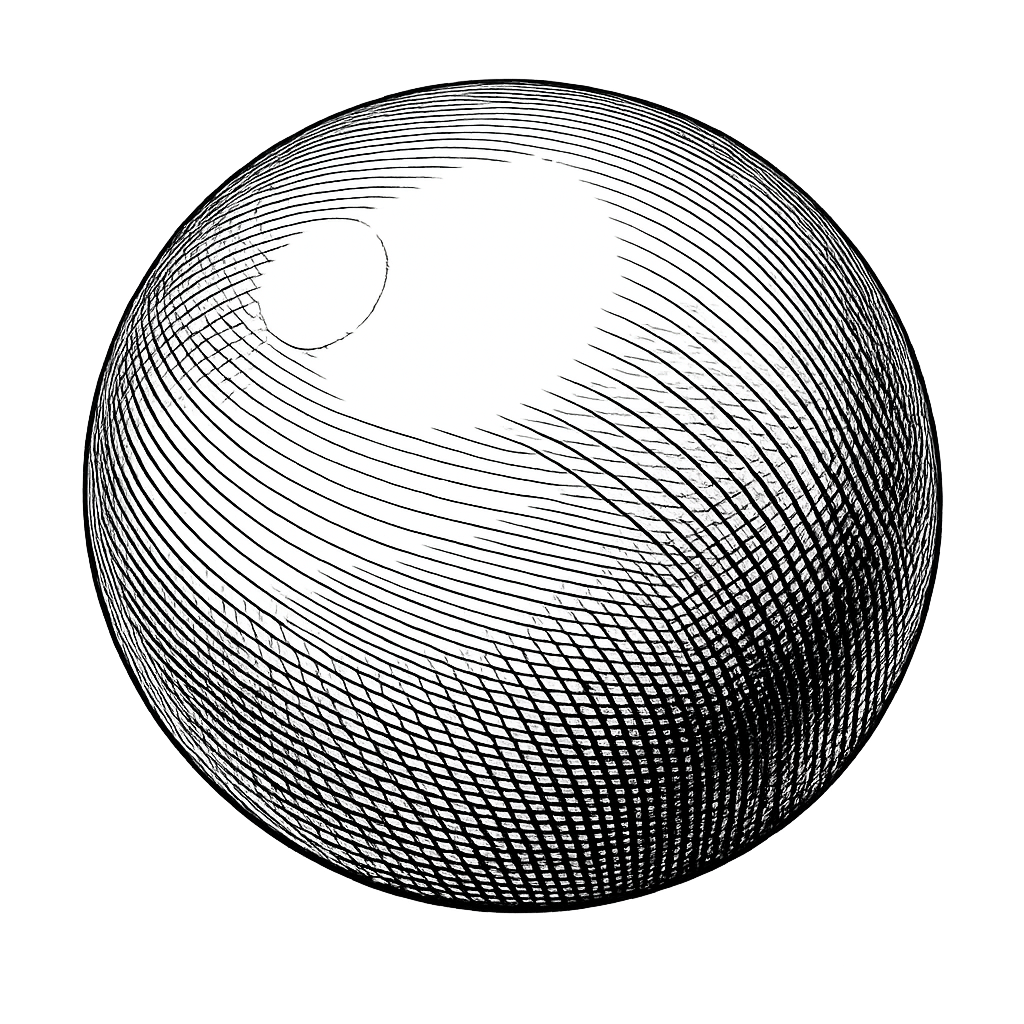
\includegraphics[width=\ew cm]{cover_ball.png}};\end{scope}}

\begin{document}
\begin{tikzpicture}[x=1cm,y=1cm]
  \useasboundingbox (0,0) rectangle (12,12);

  % ---------- Level 1: mother billiard ball (clipped round) ----------
  \begin{scope}
    \clip (4.32,7.68) circle (3.12);
    \node at (4.32,7.68) {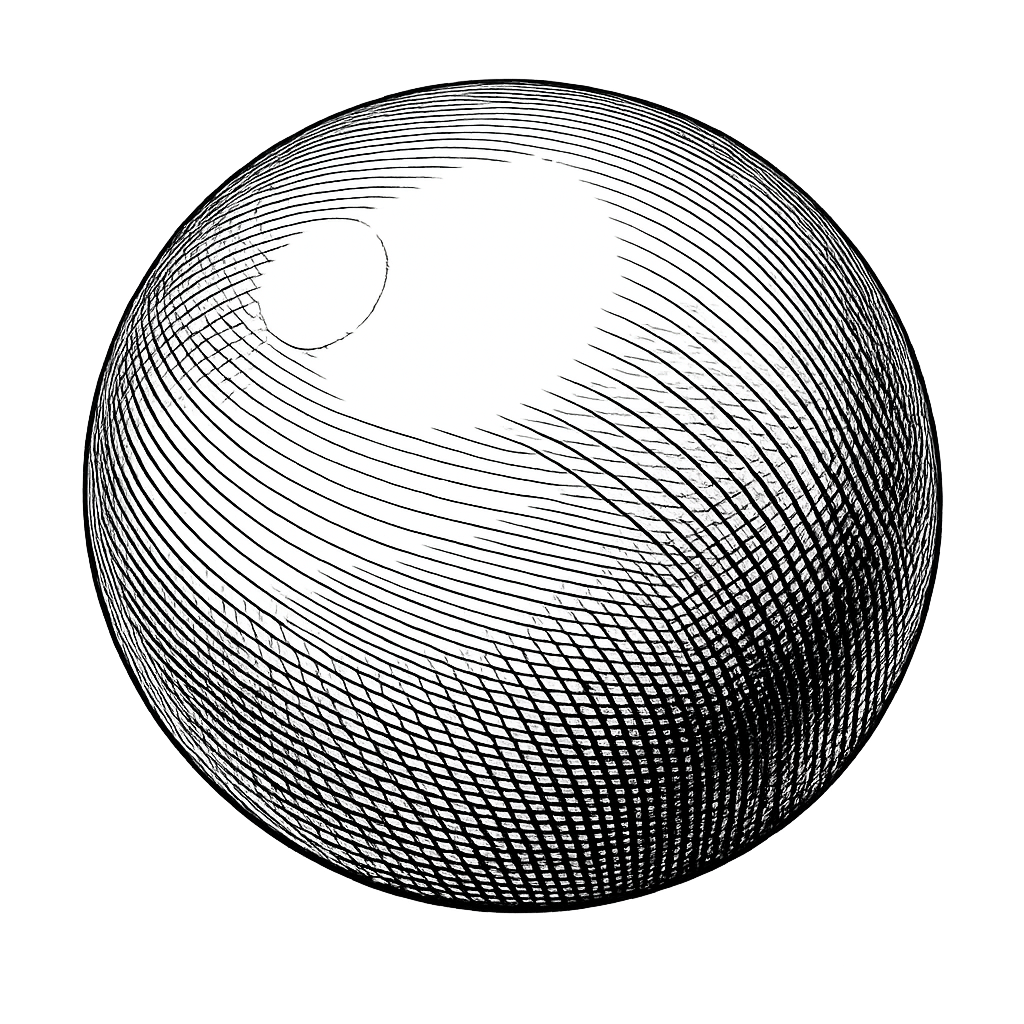
\includegraphics[width=7.3cm]{cover_ball.png}};
  \end{scope}
  % faint table-shadow: three short horizontal hatch lines under the ball
  \draw[ink,line width=0.3pt] (2.90,4.40) -- (5.74,4.40);
  \draw[ink,line width=0.3pt] (3.20,4.28) -- (5.44,4.28);
  \draw[ink,line width=0.3pt] (3.60,4.18) -- (5.04,4.18);

  % ---------- magnifier insets: Level 2 crowd, Level 3 orbit, Level 4 vortex ----------
  \inset{9.36}{6.00}{1.92}{4.0}{cover_crowd.png}
  \inset{7.44}{2.82}{1.44}{2.9}{cover_orbit.png}
  \inset{4.02}{1.38}{1.08}{2.3}{cover_vortex.png}

  % ---------- zoom cones (drawn on top; source rings mark the magnified patch) ----------
  \zoomcone{5.70}{6.78}{0.36}{9.36}{6.00}{1.92}   % mother ball -> crowd
  \zoomcone{8.52}{4.68}{0.264}{7.44}{2.82}{1.44}  % crowd -> orbit
  \zoomcone{6.52}{2.43}{0.22}{4.02}{1.38}{1.08}   % orbit -> vortex
  \zoomcone{3.34}{1.23}{0.16}{2.40}{1.02}{0.192}  % vortex -> ellipsis (cone, like the others)

  % ---------- ellipsis: the scale never bottoms out (tiny billiard balls) ----------
  \ellipball{2.40}{1.02}{0.192}
  \ellipball{1.80}{0.90}{0.132}
  \ellipball{1.38}{0.816}{0.084}
\end{tikzpicture}
\end{document}
